% !TEX root = ../Thesis.tex
\begin{document}
\documentclass[Thesis.tex]{subfiles}
\chapter{Introduction}
\label{ch:introduction}
%There are journals about case reports. -> It seems that information about individual cases is useful for doctors when reasoning about new patients. Indeed in the cognitive science literature it is documented, that humans often reason either case-based or prototype based. There is even a whole branch of AI dealing with learning to reason based on example cases, case-based reasoning.

%It seems like recommending cases similar to a current patient would be helpful for doctors for their clinical decision making. There are databases with a wealth of patient information, namely free text physician letters. However, search is limited to string matching approaches.
%-> A more elaborate automatic analysis of similarity between letters would be useful.

%For this task we obtained a small dataset from the university hospital Freiburg, on which we build a prototype of a recommender system for similar letters and explore other automatic information extraction procedures.

%--------------------------------------

\section{Motivation}

Publishing the case of a patient with a particularly interesting medical phenomenon in the form of a clinical case report has seen a change in popularity in the medical community.
%The clinical case report, a scientific publication dealing with the specifics of one particularly interesting patient, has undergone a renewal of status in the medical community. 
The number of published case reports has been declining in standard journals. This has happened not only because case reports can hardly contribute to a good impact factor, but also because their scientific benefit has been questioned \citep{Mason2001}. However, several new journals dedicated only to case reports have emerged \citep{Kidd2007}(how to cite a journal's existence, which does not have an introductory article?) and many people have argued for the value of case reports for research itself but also beyond \citep{Williams2003,Dib2008,Sandu2016}. Importantly case reports allow practitioners a more in-depth understanding of specific disease courses and provide educational material for students \citep{Nissen2014}. Although case reports lack the scientific validity of large empirical studies, it is apparent that people have strong intuitions for the usefulness of them. During our collaboration with practicing doctors we also found that practitioners use the clinical records of similar patients to guide problem solving for the current patient. Especially when faced with hard or unusual cases doctors seek similar patient information from the hospital database. While this only shows that doctors think that the presentation of similar cases helps them in their work, we will argue that this can indeed improve their medical problem solving. 

Cognitive Scientists have discussed the usefulness of examples for reasoning processes for long and found that at least in some experimental settings reasoning processes are based on earlier presented examples \citep{Medin1978}. More recently these reasoning processes have also been studied in more realistic scenarios. \citet{Klein2008} reviews models for decision making under real world circumstances. According to him experts interpret a situation based on its resemblance to remembered situations. Once a sufficiently similar situation has been retrieved from memory, experts apply the solution from the remembered situation to the current one in a thought experiment. They evaluate whether or not this solution strategy will lead to success and adjust it, if necessary. In case no way to adequately adjust the solution can be found, another situation is retrieved from memory. This process is repeated until a sufficiently good solution is found. Presentation of similar cases should therefore aid doctor's decision making in an actual clinical setting. The medical domain has also been directly addressed by research in cognitive science. \citet{Elstein2002} have concluded that for medical problem solving reasoning processes can be divided into two distinct categories. For cases perceived as easy doctors apply a kind of pattern recognition based on the examples they have encountered before and use solutions stored in memory. For harder cases, however, doctors need to rely on a more elaborate reasoning process. They have to consciously generate and eliminate hypotheses to be able to solve the problem. It is plausible that hypothesis generation as well as hypothesis falsification is also guided by the doctor's experience of earlier patients. From a more theoretical perspective \citet{Kolodner1987} have specifically argued that ``[i]ndividual experiences act as exemplars upon which to base later decisions'' in medical problem solving. Their research was partially driven by the desire to understand the way in which clinicians perform problem solving but also by the goal of building artificial systems that can aid in this process. They argue that both humans and machines can learn from specific examples and use them to reason about new problems.

Around the idea that artificial systems might learn from examples has evolved a whole branch of Artificial Intelligence (AI), which is called ``Case-based reasoning''. This domain has been greatly influenced by psychological findings, some of them mentioned above. Researchers have successfully built systems used in real world applications, that reason from the examples provided  \citep{Aamodt1994}. Within this domain of AI one of the greatest application areas is medicine. It seems that this area does not only offer straight forward usage of examples, but also has a need for automatic aids for problem solving \citep{Begum2011}.

%Indeed in cognitive science a branch of research exists that is concerned with "exemplar" or "instance"-based reasoning. In exemplar theories it is assumed that humans categorize objects based on examples stored in memory \citep{Medin1978}. However, according to \citet{Elstein2002} medical decision making can be divided into two subcategories. In cases perceived as easily solvable doctors can use pattern recognition, which can be based on previous examples, to come to a decision. In hard cases though, experts fall back to conscious hypothesis generation and elimination. We want to deal mainly with hard cases, as experts will only then seek the help of a recommender system. In those hard cases experts use hypothesis testing and therefore similar examples can provide new ideas for hypothesis formulation or help remove irrelevant or wrong hypotheses. NDM, especially RPD model asserts that experts interpret a situation based on its resemblance to an old situation, but then think the current situation through with the old strategy and see whether it would work here as well. Similar cases can show a possible, plausible strategy path and then the doctor can think it through and take this strategy or reject it based on similarity between the cases.
%Even better use Kolodner Paper!

Given the practical, psychological and theoretical reflections above we believe that it would be helpful for practitioners to be able to review cases of similar patients. One particularly well suited source for the retrieval of patient cases are databases of physician letters, as these letters provide concise summaries of the specifics of a patient that matter in practice. Search in these databases is, to our knowledge, usually limited to character matching procedures and therefore provides limited practical value for doctors. We therefore set out to build a prototypical recommender system on those physician letters to do automatic retrieval of only the relevant documents from a database.


\section{Dataset}

To get a dataset for exploratory work on the recommender system we collaborated with the university hospital Freiburg. This hospital has a database of approximately 190,000 German
physician letters in PDF form \citep{spadaro2012} (in der clinicon Beschreibung heißt es 190.000 medizinische Dokumente und Arztbriefe) (noch nicht zufrieden, wie das item in der bibliography erscheint. Ich weiß allerdings auch nicht wie es richtig wäre.). These physician letters are free text documents
written by the doctors to keep record of the patient's visit. They
usually include information about the patient's age, sex, diagnosed
diseases, therapy history, current complaints, many more medical details
like blood counts, but also personal information like names and birth dates.
The letters generally follow a rough structure. Almost all of them include a letter head (a greeting and introduction), a diagnosis (summarizing diagnosed diseases bullet point like), a therapy history (listing the past therapies with dates) and an anamnesis (free text about current complaints etc.) section, separated into individual paragraphs. In principal though, doctors are free to document this information in the way they please. The database does not, however, contain the information of 190,000 unique patients. For many patients several letters are included, as a new visit will often result in an updated letter, that is added to the database. We refer to these letters as ``follow-up'' letters.

To get permission to use a subset of those letters for our experiment, it was necessary to ensure that all personal information was removed from them. A medical student of the university hospital was therefore paid to manually anonymize 307 of the letters and forward them to us. The letters were given to us in Microsoft Word XML format.

We realized that several duplicate letters are present in this dataset, however. So to identify all of them we make use of two semi-automatic procedures for identifying duplicates. First we use a longest common subsequence string matching method. Second we represent the documents in the bag of words model, where distances between documents can be computed, and find duplicates by their proximity.


\section{The Bag of Words Model}
The bag of words model represents a text as the multiset (bag) of its words. That means all word
order information is disregarded and only the information how often a word is present in a text is encoded \citep{Manning2008vect}. (Mit der Art wie das Buch hier zitiert wird bin ich noch nicht glücklich. Es sollte eigentlich chapter 2 und 6 sein und nicht 2008 a und b.)
More concretely in the bag of words model documents are represented as fixed length
feature vectors, where every feature is a word occurrence
count. In the simplest approach every feature is the word or term frequency
tf$(t,d)$ of term $t$ in document $d$. Where tf$(t,d)$ is
the occurrence count of word or term $t$ in document $d$. To compute feature
vectors for documents in a corpus the vocabulary $V$ of the corpus
needs to be established first. Documents are represented by a $1\times|V|$
vector of the values tf$(t,d)$ for all $t\in V$.
To represent text in the bag of words model, however, the text needs to be preprocessed first.

\subsection*{Preprocessing}
In computers text is most often represented as sequences of characters. The process of extracting words from such a sequence is known as tokenization \citep{Manning2008prepr}. A first naive approach to tokenization might be to
split the sequence of characters on every whitespace and regard everything
in between as a word. This approach, however, can easily lead to unexpected
results. Consider the example string ``The doctor treats the patient.''. The naive
approach yields the words ``The'', ``doctor'', ``treats'', ``the'' and ``patient.''.
Note how the last word contains the punctuation character ``.''.
So even for very easy examples the naive approach does not produce
expected results. Luckily many more sophisticated algorithms are implemented
in ready-to-use open-source software packages.

Some words are more important or representative of a text than others and so it is a useful preprocessing step for the bag of words model to remove some frequently appearing but uninformative words, so called stop words. A list of English stop words comprises words like ``the'', ``a'', ``just'' or ``some''.  While they are necessary for the
grammatical structure of a language, they do not convey much information
about the similarity of documents \citep{Manning2008prepr}.

Additionally for the bag of words model we are not interested in the exact grammatical form in which a word is present in a text. Removing this unnecessary information is achieved with a procedure called stemming, that maps word appearances to their stem. It maps words such as ``doctors'' and ``doctor'' both to their common stem ``doctor''. Both removal of stop words and stemming seem at first glance to disregard information. This is true, but they allow to represent a text more compactly and thereby reduce the noise of the representation. The following example might provide clarification about the procedures.

\subsection*{Bag of Words Example}
Assume the corpus
consists of two documents $d_{1}=$``The patients with disease A.'' and $d_{2}=$``The patients with disease B.''. After tokenization, removal of stop words and stemming the vectors representing the two texts are:

\[
\textbf{v}_{d_1}=\begin{array}{c}
1\\
1\\
1\\
0
\end{array}\ \textbf{v}_{d_2}=\begin{array}{c}
1\\
1\\
0\\
1
\end{array}\ \begin{array}{c}
patient\\

disease\\
A\\
B\\
\end{array}
\]

Note how the punctuation character does not appear, as the tokenization has removed it from the list of words. The words ``the'' and ``with'' have been removed as stop words and the word ``patients'' has been stemmed to produce ``patient''. Then the list of words has been converted to a bag of words vector.

\subsection*{Application and shortcomings}
The vectors $v_{d_1}$ and $v_{d_2}$ live in a four dimensional vector space and we can either use them as feature vectors for a machine learning task or compute the distance between them to get a measure of dissimilarity. The standard distance measure used for bag of words vectors is the cosine distance $\rm{d_{\cos}}(v1, v2)=\frac{v1\cdot v2}{||v1||\cdot ||v2||}$, where $v1\cdot v2$ is the scalar product of $v1$ and $v2$. This distance measure is preferred over the standard euclidean distance $\rm{d_{euclid}}(v1, v2)=\sqrt{v1\cdot v2}$, as it normalizes the scalar product, by the product of the lengths of the vectors. Thereby only the relative word frequencies are important and not the absolute ones. I.e. pairs of longer documents do not have a bigger distance, just because the absolute word counts are higher. 

Generally the bag of words model has severe limitations. Consider for example
the two sentences $d_{3}=$``The patients with disease A, but not B'' and $d_{4}$=``The patients with disease B, but not A''. Their representation in the bag of words model is equivalent,
although they express quite different meanings. Still the bag of words
model is a standard approach for information retrieval problems, as
it has many desirable properties such as the fixed length representation and straight forward embedding of texts.
% In information retrieval often
%the focus lies on the topic of a text rather than it's specific content.
%Some of the weaknesses of the bag of words approach are then neglectable.
%Consider again the sentences $d_{3}$ and $d_{4}$ and additionally
%the sentence $d_{5}=$''computers automate tasks''. If we are interested
%in the topic of the sentences or in their relevance to each other,
%then the bag of words model will give the reasonable result that $d_{3}$
%and $d_{4}$ are more relevant to each other than to $d_{5}$.



\section{Dataset cleansing}

As mentioned above our initial dataset has a duplication problem. In fact two different kinds of duplicates are present in this dataset. First several letters are contained more than once. Second for several patients follow-up letters are included in the data. To ensure undistorted test results we have to identify as many of these duplicates as possible. It is clear that finding all of these duplicates manually is not only error-prone, but also very time consuming as in principle $\frac{(n-1)^2 + (n-1)}{2}$ letter comparison have to be made. With $n=307$ this amounts to almost 50,000 comparisons. Additionally personal information useful for this task like names has been removed during anonymization. We therefore explored semi-automatic aids for identifying duplicates. To verify their performance we had an expert identify all duplicates present in a subset of 150 of these letters manually.

The first method we use is based on a longest common subsequence matching procedure. We scan two documents and find the longest sequence of characters they have in common. If the length of this sequence exceeds a threshold the pair is marked as possibly duplicate and manually inspected. We lower the threshold until the false positive rate becomes to high. Secondly we preprocess all texts as described above and map them into the bag of words representation. We use the cosine distance to compute a measure of dissimilarity between pairs and mark all pairs with distance lower than a threshold as possibly duplicate and again iteratively increase the threshold.

The bag of words approach identifies all manually detected duplicates and follow-ups while having a very low false positive rate. It detects one additional manually undetected follow-up pair. The string matching procedure is not as useful due to a high false positive rate and does not detect all manually found duplicates. However, it finds a second manually undetected follow-up pair, that we have not identified with the bag of words procedure either. We use both approaches with thresholds from the "training" set on the remaining 157 letters as well. Overall we detect 18 exact copy pairs and 17 follow-up pairs. We additionally remove three letters from the dataset as they include almost no information (an artifact of the specific documentation procedure at the university hospital). This results in our final dataset consisting of 269 unique physician letters (follow-ups are only included, where mentioned explicitly).

To be able to show or hide specific parts of the letters we try to break them apart into useful sections. (Irgendwie kein runder Übergang. Bin mir auch nicht ganz sicher, ob der nächste Teil noch in die Intro gehört. Macht aber schon Sinn, dann kann ich im nächsten Kapitel gleich mit einer Anwendung anfangen, für die ich alle anderen Methoden einführen muss.)


%string matching:
%false positives = 13
%not found fu = 2
%not found copy outside 150 = 1
%not found fu outside 150 = 2


%Unfortunately 18 of the 307 letters are duplicates and thereby not usable for our
%analysis. We excluded another 3 letters, that contain almost no information
%about the patient (this kind of letter is produced due to the specific
%kind of documentation process at the clinic). Another 17 are ``follow-up''
%letters i.e. letters of the same patient at a later point in time.
%This left us with the letters of 269 individual patients (the follow-up
%letters were only used where stated explicitly). Note that it is not
%a trivial task to ensure that the set of letters contains neither
%duplicates nor follow-ups. Automated aids for this problem will be
%discussed below.

%For our goals of automatically extracting information from and finding similarities
%between the letters we additionally needed supervised information.
%For a subset of 135 letters we obtained supervised labels of two kinds.
%One, we manually labeled the letters for whether or not the patients
%suffered from specific diseases common among those patients. These
%labels were checked by an expert %Prof. Mertelsmann
%for correctness. Two, %Prof. Mertelsmann
%we obtained a grouping of these 135 patients into 50 non-overlapping groups from an expert.
%This grouping is meant to reflect the expert's
%intuition about similarities between patients, that might not be capturable
%in simple rule based grouping approaches like grouping by disease. Additionally we performed a psychological experiment with {[}replace{]} medicine students and {[}replace{]} doctors, probing their intuition about letter similarity for a larger set. With these data we tried several
%approaches for automatic extraction of information from the letters
%and automatic similarity ratings between them. The methods used in our approaches are described in the next chapter.

\section{Paragraph Extraction}

As already mentioned above, the letters almost always contain separate
paragraphs like greeting, diagnosis, therapy history and anamnesis.
To be able to hide unnecessary information or to only present requested
information it is useful to automatically extract individual
paragraphs from the documents. As the documents are similar in structure
and the word XML format allows to automatically examine the XML tree
structure of a document, we use a rule based approach for extracting
the individual paragraphs. A simplified rule to find the beginning of the diagnosis paragraph is shown in pseudocode:
%\bigskip
%
%\begin{algorithm}[H]
%	\DontPrintSemicolon
%	diagnosisRegex = '[dD]iagnose(n)?'\;
%	text = thisXmlNode.text()\;
%	\If{regex.match(text, diagnosisRegex)
%		$ {\bf and} $ boldface(text)
%		$ {\bf and} $ precededByNewline(thisXmlNode)}{
%		diagnosisStart = thisXmlNode\;
%		}
%		
%		\caption{Simplified pseudocode algorithm to find the beginning of the diagnosis paragraph}
%\end{algorithm}
%		
%\bigskip
\bigskip

\begin{lstlisting}
diagnosis_regex = '[dD]iagnose(n)?'
text = this_xml_node.text()
if diagnosis_regex.match(text)
	and boldface(text)
	and preceded_by_newline(this_xml_node):
then:
	diagnosis_start = this_xml_node
\end{lstlisting}

\bigskip
%(Weder der erste noch der zweite pseudocode gefällt mir bis jetzt. Wird noch geändert.)

A regular expression is defined that matches the beginning of the diagnosis paragraph (the German word for diagnosis is "Diagnose").
The text of every node in the XML tree is checked for a regular expression match and several other rules. If an XML node matches all criteria it is marked as the beginning of the diagnosis paragraph.
With a set of rules like the one above we automatically extract the
paragraphs of interest from the documents. This approach, however,
is not completely reliable, as the doctors are free to write the documents
in the way they please. Indeed we find several wrongly extracted paragraphs,
that e.g. include the subsequent paragraph as well. For our dataset
it is possible to check the extraction process by hand. However, this
is tedious work and is not scalable to bigger
datasets. We therefore explore whether we can in principle make use
of other automated methods to find paragraphs for which the extraction
process does not produce desired results. We therefore take several correctly extracted and one incorrectly extracted
diagnosis paragraphs and convert them to their bag of words representation.
To get a feeling for how these vectors behave we use Principle Component
Analysis (PCA) to get a lower dimensional approximation of the vectors. PCA finds the linear
subspace with desired dimensionality of the original space that preserves as much of the variance of the vectors in the original space as possible. Thereby one can gain a low dimensional approximation of the high dimensional data and use this approximation for visual inspection.
See figure \ref{fig:bow_find_odd} for a 2D PCA plot of the bag of words representation
of the correctly and incorrectly extracted diagnose paragraph. As is apparent from the figure, it would not be a
hard task to automatically detect the outlier. In this case the incorrectly
extracted paragraph includes not only the diagnosis, but also the
therapy history. In cases like this with additional text present, it is an easy task to
identify the incorrect ones. A harder problem arises, when only parts
of the paragraph of interest have been extracted. However, we believe
that this problem is of little concern. The way our rules are built it
is very unlikely that we will face this problem. The paragraph would
have to include an empty line, the subsequent one would have to contain
only boldface characters and a few more conditions would have to be
fulfilled for this problem to arise. Indeed, we did not find a case
of this problem in our dataset. (Ich könnte auch mal tatsächliche outlier detection machen, wenn du das für sinnvoll hälst. Hab ein paar Ideen, die gut funktionieren könnten, wollte aber keine Zeit rein stecken, falls wir es nicht benutzen wollen.)
\begin{figure}
	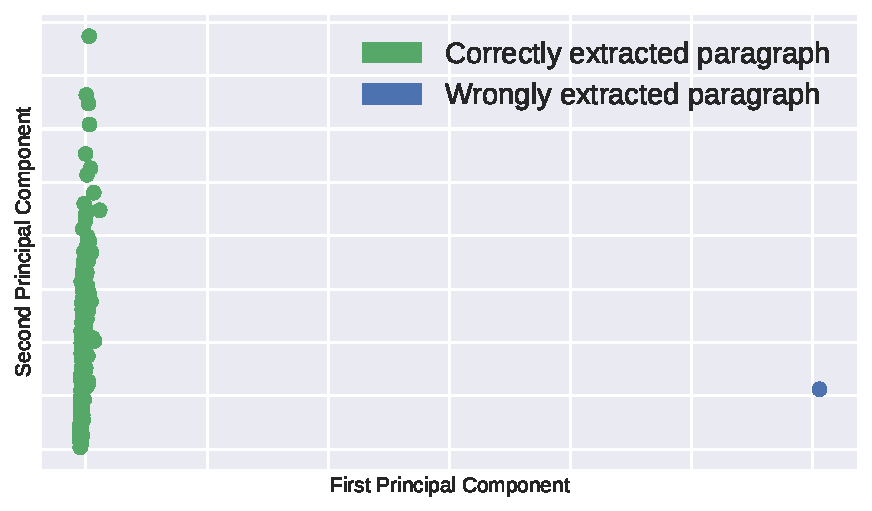
\includegraphics[width=\linewidth]{figures/bow_find_odd}
	\caption{2D PCA projection of bag of words representation of one incorrectly extracted diagnosis paragraph and several correctly extracted ones.}
	\label{fig:bow_find_odd}
\end{figure}

\end{document}